\subsection{Modellwahl}
Wie bereits erw\"ahnt, wurden f\"unf unterschiedliche Herangehensweisen betrachtet, um ein geeignetes Modell zu finden.
Eine jede dieser Herangehensweisen soll am Ende ein 'bestes' Modell liefern.
Am Ende werden dann all diese 'Gewinnermodelle' noch einmal miteinander verglichen, um ein finales Modell zu ermitteln. \\
Zun\"achst wird in Kapitel \ref{sec:wdv} auf die w\"ahrend der Untersuchung angenommene  Verteilung angegangen. 
Bevor dann die unterschiedlichen Herangehensweisen vorgestelt werden, wird die Einflussgr\"o\ss{}e \textit{region} in dem Kapitel \ref{sec:preg} genauer untersucht.

\paragraph{Wahl der Verteilung}
Wie Osgood in [Osgood2000]\footnote{Vgl.: D.Wayne Osgood: Poisson-Based Regression Analysis of Aggregate
Crime Rates, Journal of Quantitative Criminology, Vol. 16, No. 1, 2000}
schreibt, ist es von Vorteil Poissonverteilungen zu nutzen, um Kriminalit\"atsraten zu analysieren.
Poissonbasierte Regressionsmodelle sind bei Beobachtungen von Verbrechensdelikten eine gute Wahl, da sie anhand von Annahmen \"uber Fehlerverteilungen gebaut werden, die mit der Art der Ereignisanzahl konsistent sind\footnote{[Osgood2000] S.21}. \\
Osgood empfiehlt daher die Verwendung der negativen Binomialverteilung. Diese wurde von Poisson selber in den 1820-er Jahren entwickelt, um Verbrechen zu analysieren\footnote{Maltz, M. D. (1994). Operations research in studying crime and justice: Its history and accom-
plishments. In Pollock, S. M., Rothkopf, M. H., and Barnett, A. (eds.), Operations
Research and the Public Sector, Volume 6 of Handbooks in Operations Research and
Management Science, North-Holland, Amsterdam, pp. 200 - 262.}.
Daher wurde in dieser Arbeit nicht das \texttt{OLS}-Verfahren (ordinary least-squares) verwendet, welches eigentlich die Standardmethode in solchen Untersuchungen ist. \\
Eine Normalverteilung oder eine symmetrische Fehlerverteilung kann hier nicht angenommen werden, da die Verbrechensanzahl sehr gering sein kann.
Die kleinstm\"ogliche Anzahl an Verbrechen in einem County ist Null.
Daher m\"usste eine Fehlerverteilung immer mehr verzerrt werden\footnote{Vgl.: [Osgood2000] S. 21 f.}.
In Abbildung \ref{fig:nbd} sind 100 Zufallszahlen auf Basis der negativen Binomialverteilung mit $\theta = 0.7$ dargestellt.

\begin{figure}
\centering
\includegraphics[scale=0.7]{./jpgs/rnegbin.jpeg}
\caption{In beiden Diagrammen sind die relativierten Verbrechenszahlen rot dargestellt.
		 In dem linken Diagramm wurden dazu in blau mit Hilfe von \texttt{rnegbin()} berechnete     Zufallszahlen hinzugef\"ugt.
		 Das rechte Diagramm enth\"alt stattdessen zus\"atzlich Zufallszahlen, die mit \texttt{rnorm()} berechnet wurden.}
\label{fig:nbd}
\end{figure}
\par\smallskip

Um die Annahme der negativen Binomialverteilung zu rechtfertigen wurden zu Beginn der Arbeit zwei Modelle verglichen, welche die selben Daten und die selbe Formel nutzen, aber unterschiedliche Verteilungen annehmen.
Es wurde der gesamte Datensatz von allen 90 Counties genutzt.
Die verwendete Formel war:
\begin{equation}
crimes = \beta_0 \cdot prbarr:prbpris + \beta_1
\end{equation}

Un zu entscheiden, welches der Modelle besser sch\"atzt, wurden die Akaike-Werte der beiden Modelle miteinander verglichen.
In Tabelle \ref{tab:agn} finden sich diese Zahlen wieder.
Der Akaikewert von Modell \textsc{m1Nb} ist wesentlich geringer als der von \tesxtsc{m1}.
Dies sagt eigentlich nicht aus, dass \textsc{m1Nb} ein besseres Modell als \textsc{m1} ist.
Vor allem aber ist die Devienz des ersten Modells viel gr\"o\ss{}er, als die des binomialverteilten.
Dies spricht f\"ur eine deutliche Verbesserung.
\par\smallskip
W\"ahrend der Untersuchung wurden nat\"urlich mehrere Gleichungen angenommen als diese eine.
Die Ergebnisse haben aber alle zu diesem selben Schluss gef\"uhrt.
Eine graphische Veranschaulichung der Gegen\"uberstellung der beiden Verteilungen findet sich in Abbildung \ref{fig:nbd}.
Hier sieht man recht gut, dass die Verbrechenszahlen eher zu einer negativen Binomialverteilung passen, als zu einer normalen Gau\ss{}verteilung.
  
\begin{table}[ht]
\centering
\begin{tabular}{rrrr}
  \hline
 	   & df & AIC & Devienz\\ 
  \hline
	m1 & 3.00 & 1789.10 & 2118963611\\ 
  m1Nb & 3.00 & 1598.57 & 106.3874\\ 
   \hline
\end{tabular}
\caption{Gegen\"uberstellung der Akaike-Werte zweier Modelle. m1 nimmt eine Gau\ss{}verteilung an, w\"ahrend m1Nb eine negative Binomialverteilung annimmt.}
\label{tab:agn}
\end{table}


\label{sec:preg}
\paragraph{Die besondere Rolle von der Einflussgr\"o\ss{}e \textit{region}}
Bei der Einflussgr\"o\ss{}e \textit{region} handelt es sich um eine dichotome Dummy-Variable.
Sie gibt an in welchem Bereich des Bundesstaates (= die Region) sich das County befindet.
Es gibt drei m\"ogliche Werte, welche diese Variable annehmen kann: \textit{central}, \textit{west} und \textit{other}.

\begin{figure}
\centering
\includegraphics[scale=0.7, keepaspectratio,width=\textwidth,height=\textheight]{./jpgs/ncc.jpg}
\caption{Diese \"Ubersicht zeigt in etwa an wo sich die drei unterschiedlichen Regionen befinden
\footnote{https://geology.com/county-map/north-carolina.shtml, 28.03.18, 10:57} }
\label{fig:ncc}
\end{figure}

Anhand von Abbildung \ref{fig:ncc} sieht man, \"uber welche Bereiche des Bundesstaates sich diese drei Regionen erstrecken. \\
Bei der Untersuchung dieser Einflussgr\"o\ss{}e ist aufgefallen, dass diese Variable wohl hinzugef\"ugt wurde, um die st\"arker besiedelten Regionen des Bundesstaates zu kennzeichnen.
So sind die Counties, die sich z.B in der Region \textit{central} befinden wesentlich st\"arker bev\"olkert, als die Counties in der Region \textit{west}.
Die Region \textit{other} ist fl\"achenm\"a\ss{}ig die gr\"o\ss{}te, ihre Counties haben aber trotzdem eine gr\"o\ss{}ere Bev\"olkerungsdichte als die Counties der kleinsten Region \textit{west}.
Daher handelt es sich bei \textit{west} wohl auch um eine st\"arker besiedelte Region.
Dies ist deswegen interessant zu betrachten, da schon sehr fr\"uh in den Untersuchungen aufgefallen ist, dass die Variable \textit{density} sehr gut dazu geeignet ist, ein gutes Modell zu finden.

\begin{table}[ht]
\centering
\begin{tabular}{cccccc}
  \hline
  \textit{region} & Anzahl Counties & Durchschnitt \textit{crimes} & Median \textit{crimes} & \diameter \textit{density} \\ 
  \hline
    central & 34 & 4764 & 2172 & 196\\
	west & 21 & 1027 & 513  & 86\\ 
  	other & 35 & 2250 & 1235 & 101\\ 
   \hline
\end{tabular}
\caption{Vergleich der durchscnittlichen Eigenschaften der Counties aus den jeweiligen Regionen.}
\label{tab:cvp}
\end{table}

In Tabelle \ref{tab:cvp} befindet sich eine Gegen\"uberstellung der durchschnittlichen Werte von der Zielgr\"o\ss{}e \textit{crimes} und der durchschnittlichen Bev\"olkerungsdichte (\textit{density}) der drei Regionen.
Bei der Betrachtung wird ersichtlich, dass es scheinbar einen Zusammenhang zwischen \textit{region} und \textit{density} gibt.
In l\"andlichen Gegenden sind die \textit{crimes}-Werte geringer.
Befindet sich in dieser l\"andlichen Gegend aber eine gr\"o\ss{}ere Stadt, ist \textit{crimes} auch erh\"oht.

\begin{figure}
\centering
\includegraphics[scale=0.7]{./jpgs/regionc.jpeg}
 \abovecaptionskip
\caption{Anhand der Farbgebung l\"asst sich erkennen, in welchen Regionen die Counties wieviele Verbrechen gemeldet haben. Schwarz sind Counties aus der Region \textit{central}, rot die Counties aus der Region \textit{west} und gr\"un die Counties aus der Region \textit{other}.}
\label{fig:rc}
\end{figure}

\begin{figure}
\centering
\includegraphics[scale=0.7]{./jpgs/cdc.jpeg}
 \abovecaptionskip
\caption{Hier wird das Ver\"altnis \textit{density} zu \textit{crimes} aufgezeigt.}
\label{fig:cdc}
\end{figure}


In Abbildung \ref{fig:rc} wird ersichtlich, dass es in der Region \textit{central} einige Counties gibt, die wesentlich mehr Delikte gemeldet haben, als die Counties aus anderen Regionen.
Dies scheint an der h\"oheren Bev\"olkerungsdichte \textit{density} zu liegen, wie die Darstellung \ref{fig:cdc} aufzeigt. \\
Tats\"achlich wird sich herausstellen, dass diese Wechselwirkung zwischen \textit{region} und \textit{density} (also \textit{density:region}) Bestandteil von vielen guten Modellen sein wird.
Daher wurde diese Dummy-Variable nicht weiter ver\"andert.
\textsf{R} behandelt solche Variablen automatisch mithilfe von \texttt{as.factor()} als diskrete Zahlen.


\subsubsection{Herangehensweisen}
\paragraph{explorative Herangehensweise}
\par\smallskip
Um ein gutes Gef\"uhl f\"ur die Merkmalsvektoren zu bekommen, wurden zun\"achst einige Modelle ausprobiert und mittels AIC verglichen.
Damit ein Vergleichswert nach dem Akaike-Ma\ss{} vorhanden war, wurde ein komplettes Modell angenommen, das aus allen vorhandenen Merkmalen besteht. Dieses Modell hei\ss{}t \textsc{mAll}. Die entsprechende Formel sieht so aus:
\begin{equation}\begin{split}
crimes = 
\beta_0 \cdot prbarr+ \beta_1 \cdot prbpris + \beta_2  \cdot polpc +  \beta_3 \cdot density + \\
\beta_4 \cdot area + \beta_5 \cdot taxpc + \beta_6 \cdot region + \beta_7 \cdot pctmin + \\
\beta_8 \cdot pctymale + \beta_9 \cdot wcon + \beta_{10} \cdot wsta + \beta_{11} \cdot wser + \\
\beta_{12} \cdot wtrd + \beta_{13} \cdot wfir
\end{split}
\end{equation}
Es wurde bewusst darauf verzichtet in diesem 'gesamten' Modell die Intersections (Wechselwirkungen) der einzelnen Merkmale zu betrachten. Grund daf\"ur ist, dass das Akaike-Ma\ss{} Modelle mit vielen Einflussgr\"o\ss{}en mehr bestraft, als solche die weniger besitzen. Da bei dieser Untersuchung das Akaike-Ma\ss{} das am h\"aufigsten verwendete Kriterium war, sollte also das erste Modell, mit dem die anderen verglichen wurden, nicht einen gro\ss{}en negativen Wert aufweisen, so wie das in diesem Fall der Fall gewesen w\"are. (Der Akaike-Wert des Modells, das alle Merkmale und alle Wechselwirkungen zwischen diesen betrachtet, betr\"agt -3441.465. In diesem Modell gibt es 91 Freiheitsgrade.)
Die Daten \texttt{crimes.data}, welche der Funktion \texttt{glm.nb(formula, data = crimes.data)} w\"ahrend der gesamten Untersuchung gegeben wurden, wurden nicht ver\"andert. Es handelt sich hierbei immer um den gesamten Datensatz aus der Datei \textit{crimes.csv}.
\par\bigskip
Im Folgenden wurde bemerkt, dass diese Merkmale durchaus gruppiert betrachtet werden k\"onnen. Daher bestand die erste Idee darin, die unterschiedlichen Gruppierungen je Modell zu betrachten:
\par\smallskip
Die ersten beiden Merkmale (\textit{prbarr} und \textit{prbpris}) geben beide Verh\"altnisse zum Anteil aller Straft\"ater in einem County an. Daher wurden Modelle aus diesen beiden Einflussgr\"o\ss{}en betrachtet. \\
Das Modell \textsc{m1} hat den Formelaufruf \textsc{glm.nb(formula = $crimes ~ 1 + prbarr:prbpris$}.
Modell \textsc{m2} besitzt die Formel \textsc{glm.nb(formula = $crimes ~ (1 + prbarr + prbpris)^2$)}. \\
Die AIC-Werte dieser Modelle sind in Tabelle \ref{tab:sfm} einsehbar.
Wie erwartet sagen hier alle Kriterien \"Ahnliches aus:
Diese Modelle \textsc{m1} und \textsc{m2} sind sich etwas \"ahnlich, wobei das etwas komplexere Modell \textsc{m2} etwas besser abschneidet.
Beide sind aber wesentlich schlechter als das komplexe Modell \textsc{mAll}. 

\begin{table}[ht]
\centering
\begin{tabular}{rrrrr}
  \hline
 & df & AIC & SPSE & Devienz\\ 
  \hline
mAll & 17.00 & 1432.29 & 3003095120 & 92.88015 \\ 
  m1 & 3.00 & 1598.57 & 3003572113 & 106.3874\\ 
  m2 & 5.00 & 1580.94 & 3003529863 & 103.9891\\ 
   \hline
\end{tabular}
\caption{Vergleich von Modellen, die auf den Wahrscheinlichkeitsvariablen beruhen.}
\label{tab:sfm}
\end{table}

Auff\"allig in Abbildung \ref{fig:nbd} ist, dass beide Wahrscheinlichkeiten sich gewisserma\ss{}en \"ahnlich verhalten:
Die meisten Wahrscheinlichkeiten haben nur relativ geringe Verbrechensanzahlen.
Jedoch gibt es bei beiden Wahrscheinlichkeiten zwei Bereiche, in denen relativ hohe Verbrechensanzahlen vorliegen.
F\"ur die Arrestierungswahrscheinlichkeit ist dies das Intervall $[0.15, 0.3]$ und f\"ur die Verurteilungswahrscheinlichkeit liegt dieser Peak in $[0.4, 0.55]$.
Dies sind relativ geringe Wahrscheinlichkeiten.
Trotzdem ist es interessant, dass die Counties, in denen es sehr viele gemeldete Delikte gab, sich in solchen Intervallen sammeln.
Das liegt wahrscheinlich daran, dass es wahrscheinlicher ist, dass Straft\"ater 'nur' arrestiert, als gleich ganz verurteilt zu werden.
 

\begin{figure}
\centering
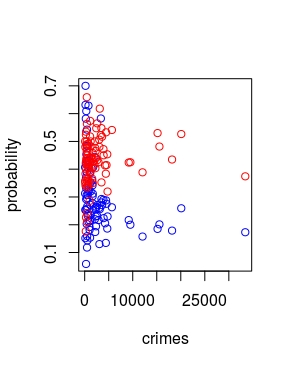
\includegraphics[scale=0.7]{./jpgs/prvc.jpeg}
\caption{Die Arrestierungswahrscheinlichkeiten sind blau gef\"arbt, w\"ahrend die Verurteilungswahrscheinlichkeiten rot gef\"arbt sind.}
\label{fig:nbd}
\end{figure}


\par\smallskip
Die Einflussgr\"o\ss{}en \textit{density} und \textit{area} sind beides r\"aumliche Merkmale. Auch sie wurden in einem Modell zusammengefasst. \\
Wie in Kapitel \ref{sec:preg} bereits erw\"ahnt wurde, liefern Modelle, welche die Variable \textit{density} verwenden, mit die besten Ergebnisse.
In diesem Zusammenhang wurde auch das dichotome Merkmal \textit{region} mit zu dieser Grupperiung gez\"ahlt. \\
Folgende Modelle, die in der unten stehenden Liste \ref{lis:spa} aufgef\"uhrt sind, wurden betrachtet.
Die Ergebnisse dieser Untersuchung liegen in Tabelle \ref{tab:spa} dar. \\
Auch hier ist die selbe Beobachtung wieder zu machen, dass, mit Zunahme der Komplexit\"at der Modelle, sich die Kriterien verbessern.

\begin{itemize}
\item \textsc{mSpatial1: glm.nb($crimes~(density+area)$)}
\item \textsc{mSpatial2: glm.nb($crimes~(density+area)^2$)}
\item \textsc{mSpatial3: glm.nb($crimes~(density+area+region)$)}
\item \textsc{mSpatial4: glm.nb($crimes~(density+area+region)^2$)}
\label{lis:spa}
\end{itemize}

\begin{table}[ht]
\centering
\begin{tabular}{rrrrr}
  \hline
 & df & AIC & SPSE & Devienz\\ 
  \hline
  mSpatial1 & 4.00 & 1462.89 & 3003028556 & 95.0647\\ 
  mSpatial2 & 5.00 & 1463.57 & 3003008479 & 95.00924\\ 
  mSpatial3 & 6.00 & 1460.37 & 3003031244 & 94.74483\\ 
  mSpatial4 & 11.00 & 1444.15 & 3003082475 & 93.6144\\ 
   \hline
\end{tabular}
\caption{\"Ubersicht der Auswertung der Modelle, welche r\"aumliche Einflussgr\"o\ss{}en benutzen.}
\label{tab:spa}
\end{table}

\par\smallskip
Die dritte Gruppierung besteht aus \textit{pctymin} (der Anteil von Minderheiten an der Gesamtbev\"olkerung) und \textit{pctymale} (der Anteil der jungen m\"annlichen Bev\"olkerung (15-24 Jahre)). 
\\
In der vierten Gruppierung wurden alle L\"ohne miteinander kombiniert. \\
Hier wurden jedoch keine weiteren Untersuchungen an der Komplexit\"atszunahme der Modelle gemacht.
Grund daf\"ur ist, dass anhand der ersten beiden Gruppierungsbetrachtungen geschlussfolgert wurde, dass komplexere Modelle auch immer die besseren Akaike-, SPSE- und Devienzwerte haben.
Ausnahme hierbei ist manchmal die Summe \"uber die erwarteten Fehlerquadrate. \\
Stattdessen wurden in diesen beiden Gruppierungen nur die jeweils komplexesten Modelle betrachtet, wie in Liste \ref{lis:pct} und Tabelle \ref{tab:pct} entnommen werden kann.


\begin{itemize}
\item \textsc{mPct: glm.nb($crimes~(pctmin+pctymale)^2$)}
\item \textsc{mTrade: glm.nb($crimes~(1+wsta+wser+wtrd+wfir)^2$)}
\label{lis:pct}
\end{itemize}

\begin{table}[ht]
\centering
\begin{tabular}{rrr}
  \hline
 & df & AIC \\ 
  \hline
mPct & 5.00 & 1612.85 \\ 
  mTrade & 12.00 & 1541.39 \\ 
   \hline
\end{tabular}
\caption{AIC-Werte der komplexen Modelle \textsc{mPct} und \textsc{mTrade}.}
\label{tab:pct}
\end{table}

\par\smallskip
Aus dieser ersten Betrachtung heraus wurde schnell klar, dass besonders die r\"aumlichen Eigenschaften gute Voraussetzungen f\"ur ein geeignetes Modell sind.
In Abbildung \ref{fig:dcc} ist ersichtlich, dass beide Gr\"o\ss{}en proportional zu einander sind und daher gut eine lineare Funktion approximiert werden kann. \\
Auch im Vergleich der Residuenplots ist ersichtlich, dass \textit{density} ein gutes Merkmal ist.
Je mehr Menschen auf engerem Raum wohnen, desto h\"oher ist die Wahrscheinlichkeit eines Verbrechens.
Dies ist insofern schon schl\"ussig, da, wenn es mehr Menschen gibt, automatisch auch gleich die Wahrscheinlichkeit h\"oher sein muss, dass es mehr Delikte gibt, als wenn es weniger Menschen g\"abe.

\begin{figure}
\centering
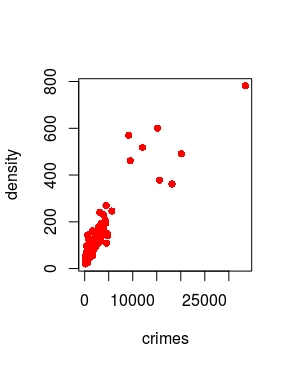
\includegraphics[scale=0.7]{./jpgs/dcc.jpeg}
\caption{Hier ist das Verh\"altnis Verbrechensanzahl / Bev\"olkerungsdichte veranschaulicht.}
\label{fig:dcc}
\end{figure}

Anhand dessen wurde ausgehend von \textsc{mSpatial4} nach weiteren Modellen gesucht, um bessere Werte zu erhalten.
Sie werden in der unten stehenden Tabelle aufgelistet.

\label{lis:pm}
\begin{enumerate}
\item \textsc{m3: glm.nb($rimes ~ 1 + area + density + area:density$)}
\item \textsc{m3Wser: glm.nb($crimes ~ 1 + area + density + area:density + wser$)}
\item \textsc{m3Opt: glm.nb($crimes ~ area + density + wser + area:density + density:wser$)}
\item \textsc{m3Opt2: glm.nb($crimes ~ area + density + wser + area:density + density:wser + prbarr + prbpris$)}
\item \textsc{m3O2: glm.nb($crimes ~ area + density + wser + prbarr + area:density + density:wser + density:prbarr + wser:prbarr + area:wser$)}
\item \textsc{mT: glm.nb($crimes ~ area + density + wser + prbarr + taxpc + area:density + density:wser + density:prbarr + wser:prbarr + area:prbarr + prbarr:taxpc$)}
\item \textsc{mR: glm.nb($crimes ~ area + density + wser + prbarr + region + area:density + density:wser + density:prbarr + wser:prbarr + area:prbarr + density:region + area:wser$)}
\end{enumerate}

\begin{figure}
\centering
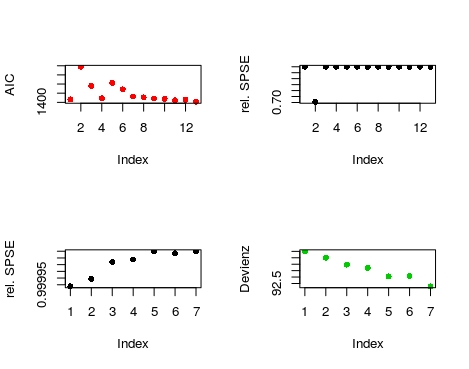
\includegraphics[scale=1]{./jpgs/assdc.jpeg}
\caption{Die Diagramme in der oberen H\"alfte zeigen jeweils die AIC-Werte (links oben) und die zueinander relativierten \hat{SPSE} (rechts oben) auf. Da es bei den \hat{assdc} einen gro\ss{}en Ausrei\ss{}er gibt, sind kaum Unterschiede ersichtlich. Daher wurden die zuletzt hinzugef\"ugten Modelle in der unteren Zeile noch einmal dargestellt. F\"ur die Indexierung der unteren Diagramme siehe \ref{lis:pm}. Die Indexierung der oberen Diagramme wird in Tabelle \ref noch einmal aufgef\"uhrt.}
\label{fig:assdc}
\end{figure}

\begin{table}[ht]
\centering
\begin{tabular}{rrrrr}
  \hline
 & Index & df & AIC & Devienz\\ 
  \hline
  1 & mAll & 17.00 & 1432.29 & 92.88015 \\ 
  2 & m1 & 3.00 & 1789.10 &  2118963611\\ 
  3 & m2 & 5.00 & 1580.94 &  103.9891\\ 
  4 & mSpatial4 & 11.00 & 1444.15 &  93.6144\\ 
  5 & mPct & 5.00 & 1612.85 &  107.5929\\ 
  6 & mTrade & 12.00 & 1541.39 &  99.01972\\ 
  7 & m3 & 5.00 & 1463.57 &  95.00924\\ 
  8 & m3Wser & 6.00 & 1454.43 &  94.50472\\ 
  9 & m3Opt & 7.00 & 1442.88 & 93.96729 \\ 
  10 & m3Opt2 & 9.00 & 1439.20 & 93.71965 \\ 
  11 & m3O2 & 11.00 & 1422.23 & 93.04977 \\ 
  12 & mT & 13.00 & 1428.82 & 93.08855 \\ 
  13 & mR & 16.00 & 1405.77 & 92.27836 \\ 
   \hline
\end{tabular}
\label{tab:assdc}
\end{table}

Bei \textsc{m3Wser} handelt es sich um die Formel, welche die selben Variablen nutzt wie \textsc{m3} und zus\"atzlich \textit{wser}.
In der Betrachtung der Einflussgr\"o\ss{}en aus \textsc{mTrade} war aufgefallen, dass \textit{wser} die beste Verbesserung mit sich bringt. \\
\textsc{m3Wser} wurde daraufhin mit Hife der Funktion \texttt{step()} optimiert.
Das daraus resultierende Modell erhielt den Namen \textsc{m3Opt}. \\
Dieses Modell wurde wiederum dadurch verbessert, indem die beiden Wahrscheinlichkeitsvariablen \textit{prbarr} und \textit{prbpris} hinzugef\"ugt wurden.
Dieses Modell erhielt den Namen \textsc{m3Opt2}. \\
Auch dieses Modell wurde unter der Verwendung von step() erweitert. Das Resultat war Modell \textsc{m3O2}.
Im n\"achsten Schritt wurde eine weitere Variable, n\"amlich \textit{taxpc} (das Pro-Kopf-Steueraufkommen), hinzugef\"ugt.
Durch diese Erweiterung wurde das Modell \textsc{mT} geschaffen. \\
Ein alternatives Modell zu \textsc{mT} soll \textsc{mR} sein: Hier wurde stattdessen \textit{region} hinzugef\"ugt. \\
\par\smallskip
Aus den Diagrammen aus Abbildung \ref{fig:assdc} kann geschlossen werden, dass durch das Hinzuf\"ugen von weiteren Variablen und anschlie\ss{}ende Optimierung die Vergleichswerte AIC und Devienz immer mehr minimieren.
Tats\"achlich verhalten sich die $\hat{SPSE}$-Werte anders.
Dies liegt wahrscheinlich daran, dass AIC und Devienz auch von der Anzahl der Einflussgr\"o\ss{}en beeinflusst werden, was bei den SPSE-Zahlen nicht der Fall ist.
\par\smallskip
Dennoch wurde sich dazu entschlossen, dass das Modell \textsc{mR} das auf diese Herangehensweise ausgesuchte Modell, das beste Modell ist.



% TODO: Diagramm der Kriterienwerte von Modellen hinzufügen, damit ersichtlich wird, dass komplexere Modelle meist die geringereren fehler haben

% TODO: zusammenfassender Residuenplot Übersicht notwendig.

\subsubsection{Vergleich aller Modelle mit jeweils nur einem Merkmal}
\label{sec:sv}
Der Ansatz bei dieser Herangehensweise ist, dass jedes Merkmal in ein einzelnes Modell gesetzt wird.
Die daraus resultierenden Modelle werden dann, wie in der ersten Herangehensweise mittels AIC, $\hat{SPSE}$ und Devienz verglichen.
Tabelle \ref{tab:asv} listet die unterschiedlichen Modelle auf und liefert besagte Kriterien, die in Abbildung \ref{fig:asv} in drei Diagrammen dargestellt werden.

\begin{table}[ht]
\centering
\begin{tabular}{rrrrrr}
  \hline
  & name & df & AIC & rel. $\hat{SPSE}$ & Devienz \\ 
  \hline
  1 & mPrbarr & 3.00 & 1584.70 & 0.999975 &  104.8274\\ 
  2 & mPrbpris & 3.00 & 1612.10 & 0.999997 & 107.9817 \\ 
  3 & mPolpc & 3.00 & 1612.10 & 0.999997 &  107.9817\\ 
  4 & mDensity & 3.00 & 1494.42 & 0.9998183 &  96.96636\\ 
  5 & mArea & 3.00 & 1611.75 & 0.9999964 &  107.9404\\ 
  6 & mTaxpc & 3.00 & 1604.40 & 0.9999852 & 107.0648 \\ 
  7 & mRegion & 4.00 & 1594.27 &  0.999976 & 105.6683\\ 
  8 & mPctmin & 3.00 & 1614.37 &  1 & 108.2571\\ 
  9 & mPctymale & 3.00 & 1609.49 & 0.99999 &  107.6686\\ 
  10 & mWcon & 3.00 & 1584.39 &  0.9999629 & 104.799\\ 
  11 & mWsta & 3.00 & 1598.82 &  0.9999806 & 106.4173\\ 
  12 & mWser & 3.00 & 1568.89 &  0.9999449 & 103.1563\\ 
  13 & mWtrd & 3.00 & 1570.84 &  0.9999284 & 103.3589\\ 
  14 & mWfir & 3.00 & 1550.43 &  0.9999175 & 101.349\\ 
   \hline
\end{tabular}
\caption{Auflistung aller Modelle, die nur eine Eingabevariable nutzen.}
\label{tab:asv}
\end{table}
 
\begin{figure}
\centering
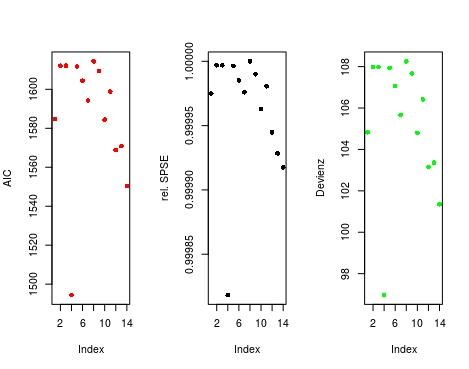
\includegraphics[scale=.7]{./jpgs/asvc.jpeg}
\caption{Veranschaulichung von Akaike-Informationsma\ss{}, $\hat{SPSE}$ und Devienz der Modelle, die jeweils nur eine Eingabevariable besitzen.}
\label{fig:asv}
\end{figure} 
 
Bei Betrachtung von Abbildung \ref{fig:asv} f\"allt auf, dass sich alle drei Kriterien \"ahnlich verhalten.
So besitzt \textsc{mDensity} (Nummer 4) in allen drei F\"allen den gerinsten Wert. \\
Dar\"uber hinaus haben die letzten Modelle, welche die L\"ohne als einzige Eingabe haben, in allen drei Ansichten die n\"achst geringeren Werte.
Hier wurde sich dazu entschieden, die Variablen \textit{density}, \textit{wser}, \textit{wsta}, \textit{wtrd} und \textit{wfir} in ein Modell \textsc{mSingles} als vorl\"aufiges Resultat zusammenzufassen. \\
Dieses Modell wurde nachtr\"aglich noch einmal mit \texttt{step()} optimiert, sodass ein weiteres Modell \textsc{mSinglesOpt} vorliegt.
In Tabelle \ref{tab:svw} wird ersichtlich, dass das beste Modell nach dieser Herangehensweise das Modell \textsc{mSinglesOpt} ist. \\
Tats\"achlich handelt es sich um ein relativ gutes Ergebnis, allerdings sind die Modelle aus der ersten Herangehensweise effektiver.

\begin{table}[ht]
\centering
\begin{tabular}{rrr}
  \hline
 & df & AIC \\ 
  \hline
mSinglesOpt & 8.00 & 1468.70 \\ 
  m3O2 & 11.00 & 1422.23 \\ 
  mR & 16.00 & 1405.77 \\ 
   \hline
\end{tabular}
\caption{AIC-Wert des Ergebnismodells durch Untersuchung der einzelnen Modelle im Vergleich zu den besten Werten aus der erste Herangehensweise.}
\label{tab:svw}
\end{table}

\subsubsection{Verwendung von step() und anschlie\ss{}ende Minimierung des Modells}
\label{sec:ste}
Hier wurde zu Beginn die Funktion \texttt{step()} mit allen m\"oglichen Eingabevariablen und all ihren Wechselwirkungen benutzt.
Dabei kam zwar ein Modell heraus, dessen Residuenplot eine Nulllinie ist, jedoch ist es so kompliziert und lang, dass es sich jeder Deutung entzieht. \\
Hier wurde ein top-down Ansatz gew\"ahlt: \\
Es wurde so fortgefahren, dass immer ein Parameter aus der Formel entfernt wurde.
Ist der AIC-Wert im Vergleich zum Vorg\"angermodell geringer, aber noch nicht so hoch wie der aus dem Modell \textsc{mSinglesOpt} oder \textsc{mR} aus den anderen Herangehensweisen, wird das gefundene Modell beibehalten, andererseits ein anderer Parameter entfernt. \\
Das auf diese Weise gefundene Modell benutzt die Formel 
\begin{equation}
crimes \sim density + area + pctmin + wsta + density:area + density:pctmin
\end{equation}
als Formelaufruf. 
\par\smallskip

Abbildung \ref{fig:sc} zeigt den Verlauf der Minimierung der AIC-Werte.
Das Verfahren wurde 14 mal ausgef\"uhrt.
Interessant in Abbildung \ref{fig:sc} ist der gro\ss{}e Sprung nach der vierten Iteration.
Bis dahin wurden die Einflussgr\"o\ss{}en \textit{prbarr}, \textit{prbpris}, \textit{region} und \textit{polpc} entfernt. 

\begin{figure}
\centering
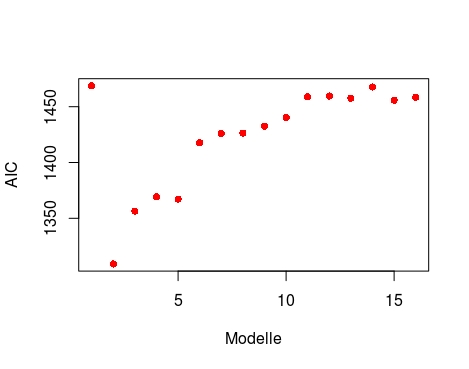
\includegraphics[scale=.7]{./jpgs/sc.jpeg}
\caption{Veranschaulichung von Akaike-Informationsma\ss{}, $\hat{SPSE}$ und Devienz der Modelle, die jeweils nur eine Eingabevariable besitzen.}
\label{fig:sc}
\end{figure} 

\begin{table}[ht]
\centering
\begin{tabular}{rrr}
  \hline
 & df & AIC \\ 
  \hline
mSinglesOpt & 8.00 & 1468.70 \\ 
  m1 & 77.00 & 1309.12 \\ 
  m2 & 63.00 & 1356.44 \\ 
  m3 & 50.00 & 1369.25 \\ 
  m4 & 38.00 & 1367.22 \\ 
  m5 & 28.00 & 1417.72 \\ 
  m6 & 23.00 & 1425.96 \\ 
  m7 & 20.00 & 1426.40 \\ 
  m8 & 17.00 & 1432.59 \\ 
  m9 & 14.00 & 1440.23 \\ 
  m10 & 11.00 & 1458.83 \\ 
  m11 & 10.00 & 1459.56 \\ 
  m12 & 9.00 & 1457.60 \\ 
  m13 & 8.00 & 1467.60 \\ 
  m14 & 8.00 & 1455.82 \\ 
  m15 & 8.00 & 1458.50 \\ 
   \hline
\end{tabular}
\caption{Die Modelle sind hier nach ihrer Iteration benannt.}
\end{table}
 
\subsubsection{Verwendung von cor()}
Analog zu Kapitel \ref{sec:sv} wurden hier die Korrelationen zwischen der Zielvariable \textit{crimes} und den einzelnen Eingabevariablen mithilfe von \textt{cor()} berechnet.
Daraus resultieren Tabelle \ref{tab:cor} und Abbildung \ref{fig:cor}.
In dieser Abbildung ist eine etwas gr\"o\ss{}ere L\"ucke in dem Intervall $[0.2, 0.309]$.
Alle Werte dar\"uber wurden in das 'Siegermodell' eingetragen.
Daraus resultiert ein Modell mit dem Formelaufruf:
\begin{equation}
crimes \sim (density+wser+wfir+wtrd+pctymale)
\end{equation} 
Bei der Betrachtung von Tabelle \ref{tab:co2} f\"allt auf, dass kein sehr gutes Modell gefunden wurde.
Dies liegt daran, dass hier keine Wechselwirkungen zwischen den Eingabeparametern beachtet wurden.
Interessant ist aber zu sehen, dass dadurch hier einige Parameter aus der Lohn-Gruppierung hinzugef\"ugt wurden, die in den anderen Herangehensweisen, wo die Wechselwirkungen betrachtet wurden, nicht hinzugef\"ugt wurden.

\begin{table}[ht]
\centering
\begin{tabular}{rrr}
  \hline
  # & name & Korrelation mit \textit{crimes} \\ 
  \hline
  1 & mPrbarr & -0.2994541\\ 
  2 & mPrbpris & -0.008989058 \\ 
  3 & mPolpc & -0.008989058\\ 
  4 & mDensity & 0.9091849\\ 
  5 & mArea & 0.1170337\\ 
  6 & mTaxpc &  0.2002482\\ 
  7 & mRegion & 0.03044025\\ 
  8 & mPctmin & 0.03044025\\ 
  9 & mPctymale & 0.1690798\\ 
  10 & mWcon & 0.4683103\\ 
  11 & mWsta & 0.3094517\\ 
  12 & mWser & 0.4995101\\ 
  13 & mWtrd & 0.623725\\ 
  14 & mWfir & 0.5460246\\ 
   \hline
\end{tabular}
\caption{Auflistung aller Korrelationen der Eingabevariablen mit \textit{crimes}.}
\label{tab:cor}
\end{table}

\begin{figure}
\centering
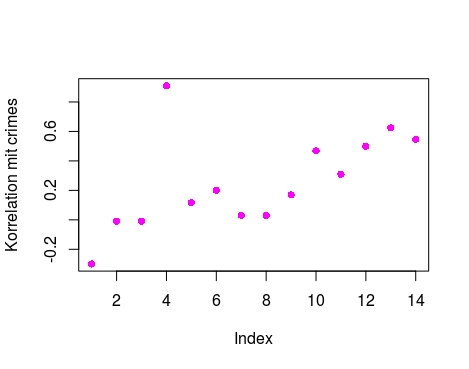
\includegraphics[scale=.7]{./jpgs/corc.jpeg}
\caption{Graphische Veranschaulichung der verschiedenen Korrelationswerte.}
\label{fig:cor}
\end{figure} 

\begin{table}[ht]
\centering
\begin{tabular}{rrr}
  \hline
 & df & AIC \\ 
  \hline
mCor & 7.00 & 1472.06 \\ 
  mCor mit step() optimiert & 9.00 & 1456.20 \\ 
  mR & 16.00 & 1405.77 \\ 
   \hline
\end{tabular}
\caption{Vergleich der Modelle mit dieser Herangehensweise mit dem besten Modell aus der ersten Herangehensweise.}
\label{tab:co2}
\end{table}

\subsubsection{Die Gewinnermodelle}
Tats\"achlich schneidet im Vergleich zu den anderen drei Herangehensweisen die explorative am besten ab, wie anhand von Tabelle \ref{tab:wic} und Abbildung \ref{fig:wic} nachvollzogen werden kann.
Dies liegt aber auch vor allem daran, dass \textsc{mExplorativ} die geringste Anzahl an Eingabevariablen besitzt.

\begin{table}[ht]
\centering
\begin{tabular}{rrrrrr}
  \hline
  & name & df & AIC & $\hat{SPSE}$ & Devienz  \\ 
  \hline
	1 & mExplorativ & 16.00 & 1405.77 & 0.9999914 & 92.27836 \\ 
	2 & mEinzeln & 8.00 & 1468.70 &  0.999921 & 94.33151\\   
  	3 & mStep & 9.00 & 1457.60 &  1 & 94.97083\\ 
    4 & mCor & 7.00 & 1472.06 &  0.9999654 & 95.23178\\ 
   \hline
\end{tabular}
\caption{Kriterien der vier Gewinnermodelle}
\label{tab:wic}
\end{table}

\begin{figure}
\centering
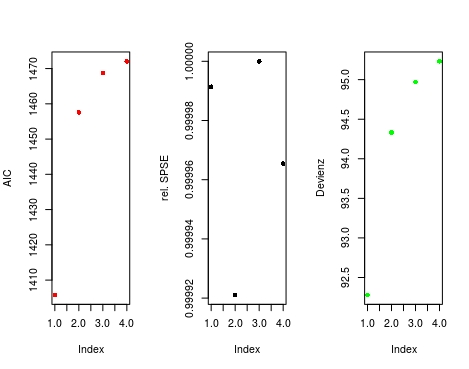
\includegraphics[scale=1]{./jpgs/wic.jpeg}
\caption{Graphische Veranschaulichung der verschiedenen Korrelationswerte.}
\label{fig:wic}
\end{figure} 
\newpage 
\subsection{Simulationsaufgabe}
\paragraph{Beschreibung simulation()}
\paragraph{Auswertung der Ergebnisse}
\subparagraph{einfaches Modell: \textit{mDensity}}
\subparagraph{Ergebnisse mit Gewinnermodell aus der ersten Aufgabe}
Hier leite ich zur Diskussion \"uber.